\section{The split-quintic transition}\label{sec:quintic}

We calculate the global data for Theorem~\ref{thm:integrated}, including
the integral information that is not visible in the Hodge-number change.
The geometric transition is classical \cite{greene-morrison-strominger};
the following argument fixes the markings and attachment conventions
used in this application.
The calculation follows the distinction made for compact K3 bundle
moduli in \cite{wuebben-reconstruction,wuebben-attachments}: local
fillings must be combined with global complement and attachment data.
Here integral Lefschetz, the projective intersection form and the Thom
sequences determine those data from \eqref{eq:split-equations}.

\subsection{The genuine global family}
Choose independent linear forms $l_1,l_2$ and general quartics $q_1,q_2$
on $\PP^4$, and set
\begin{equation}\label{eq:split-equations}
 \begin{split}
 F_0&=l_1q_2-l_2q_1,\qquad X_0=\{F_0=0\},\\
 Y&=\{ul_1+vl_2=0,\ uq_1+vq_2=0\}
       \subset\PP^4\times\PP^1,\\
 X_t&=\{F_0+tG=0\}.
 \end{split}
\end{equation}
Here $G$ is a quintic nonzero at the sixteen points of
$q_1=q_2=0$ in $\Pi=\{l_1=l_2=0\}$. The precise open conditions
are transversality of the two restricted quartics, smoothness of $X_0$
off $\Pi$, and smoothness of $Y$.

\begin{proposition}\label{prop:split-existence}
These conditions hold on a nonempty open set. The projection $q:Y\to X_0$
is a projective small crepant resolution of exactly sixteen ordinary
nodes. After shrinking the parameter disc, \eqref{eq:split-equations}
is a flat polarized family with trivial relative canonical bundle and
all noncentral fibres smooth. Every node is smoothed to first order.
Both $Y$ and $X_t$ are simply connected.
\end{proposition}
\begin{proof}
The linear system $l_1q_2-l_2q_1$ is the full degree-five ideal of $\Pi$
and is basepoint free off $\Pi$, so Bertini gives smoothness there.
On $\Pi$ its differential is $q_2dl_1-q_1dl_2$. General plane quartics
meet transversely in sixteen points by B\'ezout. At each intersection,
$(l_1,l_2,q_1,q_2)$ are analytic coordinates: the first two are normal
to $\Pi$ and the last two are independent along it. The local equation
is the quadratic determinant, an ordinary double point.

The incidence divisor $ul_1+vl_2=0$ is smooth, including over $\Pi$,
where its normal differential $u\,dl_1+v\,dl_2$ is nonzero. The second
sections $uq_1+vq_2$ form a basepoint-free system there. Bertini gives
smooth $Y$. Projection has a unique kernel line at rank-one matrices
and a whole $\PP^1$ at the sixteen rank-zero matrices. The determinant
coordinates identify its local resolution with
$\OO_{\PP^1}(-1)^{\oplus2}$. Adjunction for the two ample divisor
classes $H+L$ and $4H+L$ gives $K_Y=0$.

The relative hypersurface is flat over a sufficiently small disc.
The condition $G(p_i)\ne0$ gives a simple local smoothing; equivalently
the holomorphic Morse lemma applies to $F_0/G$. Outside the node
neighborhoods, compactness prevents a sequence of critical points from
approaching the smooth central exterior. Thus all sufficiently small
nonzero fibres are smooth. Adjunction gives trivial relative canonical
bundle. Ehresmann's theorem with transverse boundary identifies the
exteriors. Finally integral Lefschetz, twice for $Y$ and once for the
smooth quintic, gives simple connectivity and the integral degree-two
markings used below.
\end{proof}

\begin{figure}[!b]
 \centering
 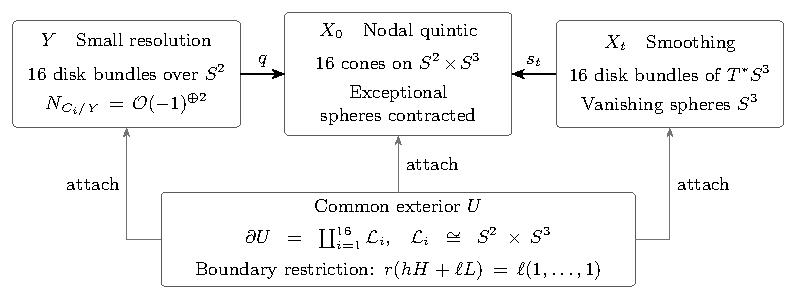
\includegraphics[width=\textwidth]{figures/output/fig01_transition.pdf}
 \caption{The common exterior and its three fillings. The map $q$ is
 algebraic; $s_t$ is the continuous Milnor collapse along the chosen ray.
 The resolution and smoothing cores have real dimensions two and three.
 The same boundary restriction gives the vanishing-cycle relation and
 the periods in the spectral coefficient.}
 \label{fig:transition}
\end{figure}

\subsection{The full integral rings}
Let $H,L$ be the hyperplane classes of $\PP^4,\PP^1$ restricted to $Y$.
Lefschetz gives $H_2(Y;\ZZ)=\ZZ^2$ and $H_2(X_t;\ZZ)=\ZZ$.
Together with $H_1=0$, universal coefficients and integral Poincar\'e
duality imply torsion-freeness in every degree. The fundamental class
of $Y$ in the product is $(H+L)(4H+L)$, whence
\begin{equation}\label{eq:split-cubic}
 \int_YH^3=5,\qquad \int_YH^2L=4,\qquad L^2=0.
\end{equation}
Take $A,B\in H^4(Y;\ZZ)$ dual to $H,L$, and let
$a_4\in H^4(X_t;\ZZ)$ satisfy $\int_{X_t}Ha_4=1$. Then:

\begin{table}[tb]
\centering
\caption{Integral cohomology and characteristic data of the compact fibres.}
\label{tab:integral-rings}
\begin{adjustbox}{max width=\textwidth,center}
\begin{tabular}{ll@{\hspace{1.5em}}l}
\toprule
 & $Y$ & $X_t$\\
\midrule
$H^2$ & $\ZZ H\oplus\ZZ L$ & $\ZZ H$\\
$H^4$ & $\ZZ A\oplus\ZZ B$ & $\ZZ a_4$\\
Degree-two products & $H^2=5A+4B$, $HL=4A$, $L^2=0$ & $H^2=5a_4$\\
Top products & $HA=LB=[\mathrm{pt}]$, $HB=LA=0$ & $Ha_4=[\mathrm{pt}]$\\
$\operatorname{rank}H^3$ & $174$ & $204$\\
$c_2$ & $50A+24B$ & $50a_4$\\
Euler characteristic & $-168$ & $-200$\\
\bottomrule
\end{tabular}
\end{adjustbox}
\end{table}

To verify the characteristic numbers directly, use
\[
 c(TY)=\frac{(1+H)^5(1+L)^2}{(1+H+L)(1+4H+L)}.
\]
This gives $c_2(Y)=6H^2+5HL$ and
$c_3(Y)=-20H^3-17H^2L$. For a quintic,
$c_2=10H^2$ and $c_3=-40H^3$. Since $H^1=H^5=0$, the Euler
numbers give the displayed third Betti numbers. The degree-three product
on each compact fibre is its unimodular alternating pairing times the
point class. With $H^0=H^6=\ZZ$, these statements specify the full rings
up to symplectic basis choices. The product subgroup generated by
$H^2$ and $HL$ in $H^4(Y)$ has index
$|\det\left(\begin{smallmatrix}5&4\\4&0\end{smallmatrix}\right)|=16$;
it is not an integral basis.

Every exceptional curve has degrees $(H\cdot C_i,L\cdot C_i)=(0,1)$.
They therefore represent the same primitive homology class $c_Y$, with
Poincar\'e dual $B$. Primitivity follows from the period of $L$.

\subsection{The common exterior and all cohomological attachments}
Remove disjoint tubular neighborhoods of the exceptional curves, obtaining
a compact exterior $U$. Its boundary components $\mathcal L_i$ are
$S^2\times S^3$. Define
\[
 \Lambda=\ZZ^{16},\quad \mathbf1=(1,\ldots,1),\quad
 \Lambda_0=\ker(\Sigma:\Lambda\to\ZZ),\quad W=\Lambda/\ZZ\mathbf1.
\]
The homological Thom sequence uses
$H_j(Y,U)=H_{j-4}(\coprod C_i)$.
The maps $H_4(Y)\to\Lambda$ and $H_6(Y)\to\Lambda$ have primitive
diagonal image: the former is exceptional intersection, witnessed by
$L\cdot C_i=1$, and the latter is the oriented diagonal fundamental
class. Thus $U$ has free integral homology and cohomology, with Betti
vector
\begin{equation}\label{eq:exterior-betti}
 (1,0,2,189,1,15,0),
\end{equation}
and exact sequences
\begin{equation}\label{eq:exterior-homology}
 0\to W\to H_3(U)\to H_3(Y)\to0,
 \qquad 0\to H_3(U)\to H_3(X_t)\to \Lambda_0\to0.
\end{equation}
The second comes from the Milnor fillings, whose cores are three-spheres.
The vanishing spheres span $W$, with relation
$\delta_1+\cdots+\delta_{16}=0$. Both successive quotients in
\eqref{eq:exterior-homology} are free; hence $W$ embeds primitively in
$H_3(X_t)$, and is isotropic because the spheres are disjoint.

In cohomology the Thom sequence kills exactly $\ZZ B$ in degree four.
Writing $\bar A=A|_U$, the even products are
\[
 H^2=5\bar A,\qquad HL=4\bar A,\qquad L^2=0.
\]
Orient each link as a boundary component of $U$ and choose generators
$\alpha_i\in H^2(\mathcal L_i)$ and $\beta_i\in H^3(\mathcal L_i)$
with $L|_{\mathcal L_i}=\alpha_i$ and $\int\alpha_i\beta_i=1$.
The symbol $\beta_i$ here has degree three; the harmonic degree-two
form remains $\vartheta_i$. The degree-three restriction is
\begin{equation}\label{eq:exterior-cohomology}
 0\to H^3(Y)\to H^3(U)\xrightarrow{r_U}\Lambda_0\to0,
\end{equation}
and degree-five restriction is the inclusion $H^5(U)=\Lambda_0\hookrightarrow\Lambda$.
Boundary multiplicativity and that injectivity imply, for $y\in H^3(U)$,
\[
 Hy=0,\qquad Ly=r_U(y)\in \Lambda_0=H^5(U).
\]
All degree-six products vanish. These formulas give the entire exterior
ring, without supplying an unspecified multiplication as additional input.

For completeness, use the Mayer--Vietoris difference $j_U^*-j_F^*$.
Let $x_i$ be the degree-two generator of the resolution filling and $z_i$
the degree-three generator of the smoothing filling, restricting to
$\alpha_i,\beta_i$. The nonzero difference maps are:
\begin{center}
\begin{adjustbox}{max width=\textwidth,center}
\begin{tabular}{cll}
\toprule
Degree & Resolution & Smoothing\\
\midrule
$0$ & $c_0\mathbf1-(c_i)$ & $c_0\mathbf1-(c_i)$\\
$2$ & $\ell\mathbf1-(x_i)$ & $\ell\mathbf1$\\
$3$ & $r_U(y)$ & $r_U(y)-(z_i)$\\
$5$ & $\Lambda_0\hookrightarrow\Lambda$ & $\Lambda_0\hookrightarrow\Lambda$\\
\bottomrule
\end{tabular}
\end{adjustbox}
\end{center}
Here $hH+\ell L$ is the exterior degree-two class, $c_0$ is an exterior
constant, and $(c_i)$ are filling constants.
The nonzero connecting maps are
\begin{equation}\label{eq:connecting-maps}
 \begin{aligned}
 \partial_Y^3(v)&=(\Sigma v)B,&
 \partial_Y^5(v)&=(\Sigma v)[\mathrm{pt}],\\
 \partial_{X_t}^2&:\Lambda\twoheadrightarrow W\hookrightarrow H^3(X_t),&
 \partial_{X_t}^5(v)&=(\Sigma v)[\mathrm{pt}].
 \end{aligned}
\end{equation}
All other connecting maps vanish. The signs follow by representing the
connecting class on an outward-$U$ collar by $d\chi_F\wedge\eta$,
where $\chi_F$ increases toward the filling. Pairing the degree-three
connecting class of $\beta_i$ with $H,L$ gives zero and one respectively,
hence $+B$. The same collar integral gives the top-degree sum maps.

Restriction from $Y$ preserves $H,L$, sends $(A,B)$ to $(\bar A,0)$,
and identifies $H^3(Y)$ with $\ker r_U$. Restriction from $X_t$ sends
$(H,a_4)$ to $(H,\bar A)$ and surjects $H^3(X_t)\to H^3(U)$ with
kernel the cohomological copy of $W$ in \eqref{eq:connecting-maps}.
Restriction to each Milnor filling is the corresponding component of
$r_U(y)$. These data specify the full integral cohomological attachment
diagram; no homotopy classification of the attaching maps is asserted.

\subsection{Monodromy and specialization}\label{sec:specialization}
Use left Poincar\'e duals in odd degree, characterized by
$\int\PD_L(\delta)\wedge\eta=\int_\delta\eta$, and orient $\delta_i$
so that $\PD_L(\delta_i)=\partial_{X_t}^2(\alpha_i)$.
For a positive simple loop, the Picard--Lefschetz transformation has
$N=T-I$, $N^2=0$, and, up to the common intersection-sign convention,
\begin{equation}\label{eq:monodromy}
 N\gamma=\pm\sum_{i=1}^{16}\langle\gamma,\delta_i\rangle\delta_i.
\end{equation}
Equivalently it factors through
$H_3(X_t)\to \Lambda_0\hookrightarrow\Lambda\twoheadrightarrow W$.
In the bases $e_i-e_{16}$ of $\Lambda_0$ and $\delta_1,\ldots,\delta_{15}$
of $W$, the nonzero block is $\pm(I_{15}+J_{15})$, where $J_{15}$
is the all-ones matrix. Its Smith form is
$\operatorname{diag}(1^{14},16)$: subtracting the first row from the
others gives fourteen unit pivots, and the remaining determinant is
sixteen. Thus the monodromy image has index sixteen in the primitive
vanishing lattice. This relation-matrix description is consistent with
the general conifold monodromy calculation of \cite{lee-lin-wang}.

The contraction $q:Y\to X_0$ collapses each exceptional sphere to its
node. Along the chosen smoothing ray, the Milnor collapse
$s_t:X_t\to X_0$ collapses each vanishing sphere. A disk cotangent bundle
of $S^3$ modulo its zero section is the cone on its sphere bundle; the
local collapses glue to the common exterior identification. Both maps
have degree one. Collapsing the sixteen cores to their distinct nodes
identifies the corresponding relative pairs with $(X_0,\{p_i\})$.
In degrees at least two its relative groups are $H_j(X_0)$. The pair
sequences give
\begin{equation}\label{eq:central-homology}
 \begin{split}
 &0\to H_3(Y)\xrightarrow{q_*}H_3(X_0)\to \Lambda_0\to0,\\
 &0\to W\to H_3(X_t)\xrightarrow{s_{t*}}H_3(X_0)\to0.
 \end{split}
\end{equation}
In degree two, $q_*$ is the quotient by $\ZZ c_Y$ and $s_{t*}$ is
an isomorphism. In degree four, $q_*$ is an isomorphism and $s_{t*}$
is a primitive injection with free rank-one cokernel. To see the latter,
the full relative sequence is
\[
 0\to H_4(X_t)\to H_4(X_0)\to\Lambda
 \xrightarrow{e_i\mapsto\delta_i}H_3(X_t)\to H_3(X_0)\to0,
\]
and the middle kernel is $\ZZ\mathbf1$. All central groups are free,
with Betti vector $(1,0,1,189,2,0,1)$. The maps are isomorphisms in
degrees zero and six; degrees one and five vanish.

The first sequence of \eqref{eq:exterior-homology} maps to the second
sequence of \eqref{eq:central-homology}, with identity on $W$, exterior
inclusion in the middle, and $q_*$ on the right. Both vertical cokernels
are canonically $\Lambda_0$. This is naturality of the actual collapse maps,
rather than an arbitrary splitting of free groups.

Let $h\in H^2(X_0)$ be the central polarization and choose
$A_0,B_0\in H^4(X_0)$ by $q^*(h,A_0,B_0)=(H,A,B)$.
The central even products and smoothing pullback are
\begin{equation}\label{eq:central-ring}
 h^2=5A_0+4B_0,\quad hA_0=[\mathrm{pt}],\quad hB_0=0,
 \qquad s_t^*(h,A_0,B_0)=(H,a_4,0).
\end{equation}
Indeed pairing the degree-four pullbacks with $H$, and using degree one,
fixes their coefficients integrally. Dually the image of $s_{t*}$ in
degree four is $\ZZ q_*\PD_Y(H)$. In degree three $q^*$ is surjective
with primitive kernel $\Lambda_0^*\simeq W$, and $s_t^*$ is a primitive injection
onto the annihilator of the vanishing homology lattice. Since $\im N$
has finite index in $W$, an integer-valued homomorphism annihilates
$\im N$ exactly when it annihilates $W$. Thus
\[
 \im s_t^*=\ker(T^*-I)\subset H^3(X_t;\ZZ).
\]
The central degree-three cup pairing factors through $q^*$ and the
unimodular pairing of $Y$, by naturality and degree one. Its radical is
$\ker q^*$; the Milnor pullback takes that radical to the primitive
vanishing cohomology lattice by naturality of the connecting map.
These formulas specify the central ring, including its degenerate
middle pairing, without assuming ordinary Poincar\'e duality for $X_0$.

\subsection{The spectral coefficient and the allowed parameters}
Proposition~\ref{prop:split-existence} and Table~\ref{tab:integral-rings}
verify all hypotheses of Theorem~\ref{thm:main}. Taking $D=L$ gives
\[
 M=\frac{4^2}{5}-0=\frac{16}{5},\qquad
 \frac{2\pi\sum_{i=1}^{16}(L\cdot C_i)^2}{M}=10\pi,
\]
which proves the spectral assertion of Theorem~\ref{thm:integrated}.
By Proposition~\ref{prop:restriction-spectrum}, the vector
$(L\cdot C_i)_i=\mathbf1$ in this calculation is the same vector
that generates the kernel of the vanishing-cycle map. The denominator
is the polarized primitive norm from the same integral ring. It is
not an independent local coefficient fitted to the spectrum.

The family has one exceptional-area direction. Arbitrary independent
node parameters are not implied by the number of nodes. Already at
first order, evaluation of quintics at the sixteen planar points has
rank fifteen: the degree-five Hilbert function of a plane $(4,4)$
complete intersection is $\binom72-2\binom32=15$.
Cayley--Bacharach makes the unique evaluation relation nonzero at every
point. The actual pencil selects a compatible vector nonzero at all
nodes. This is sufficient for the fixed-ray theorem and does not
supply uniformity for arbitrary independent smoothing rates.
